% Oblique, orthographic vector construction. Solid/dashed lines encode state.
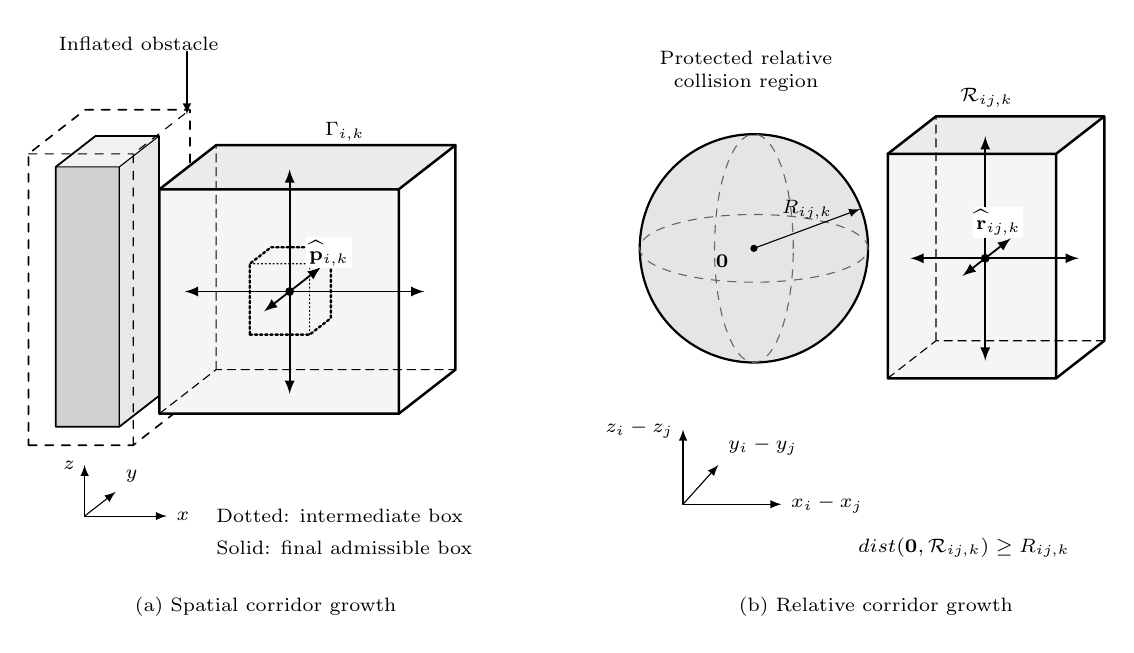
\begin{tikzpicture}[x=1cm,y=1cm,>=latex,font=\fontsize{7}{8}\selectfont,line cap=round,line join=round]
% Panel A: true 3-D cuboids in an explicit oblique basis.
\node[anchor=north,font=\fontsize{7}{8}\selectfont] at (2.3,-1.95) {(a) Spatial corridor growth};
\begin{scope}[x={(.95cm,0cm)},y={(.36cm,.28cm)},z={(0cm,1cm)}]
% Inflated obstacle: solid core and dashed clearance boundary.
\fill[black!18] (-.5,.3,0)--(.35,.3,0)--(.35,.3,3.3)--(-.5,.3,3.3)--cycle;
\fill[black!9] (.35,.3,0)--(.35,1.7,0)--(.35,1.7,3.3)--(.35,.3,3.3)--cycle;
\fill[black!5] (-.5,.3,3.3)--(.35,.3,3.3)--(.35,1.7,3.3)--(-.5,1.7,3.3)--cycle;
\draw[line width=.65pt] (-.5,.3,0)--(.35,.3,0)--(.35,1.7,0)--(.35,1.7,3.3)--(-.5,1.7,3.3)--(-.5,.3,3.3)--cycle;
\draw (.35,.3,0)--(.35,.3,3.3)--(.35,1.7,3.3) (-.5,.3,3.3)--(.35,.3,3.3);
\draw[dashed,line width=.6pt] (-.75,0,-.15)--(.65,0,-.15)--(.65,2,-.15)--(.65,2,3.55)--(-.75,2,3.55)--(-.75,0,3.55)--cycle;
\draw[dashed] (.65,0,-.15)--(.65,0,3.55)--(.65,2,3.55) (-.75,0,3.55)--(.65,0,3.55);
% Final corridor.
\fill[black!4] (1,0,.25)--(4.2,0,.25)--(4.2,0,3.1)--(1,0,3.1)--cycle;
\fill[black!8] (1,0,3.1)--(4.2,0,3.1)--(4.2,2,3.1)--(1,2,3.1)--cycle;
\draw[line width=.9pt] (1,0,.25)--(4.2,0,.25)--(4.2,2,.25)--(4.2,2,3.1)--(1,2,3.1)--(1,0,3.1)--cycle;
\draw[line width=.9pt] (4.2,0,.25)--(4.2,0,3.1)--(4.2,2,3.1) (1,0,3.1)--(4.2,0,3.1);
\draw[densely dashed] (1,0,.25)--(1,2,.25)--(4.2,2,.25) (1,2,.25)--(1,2,3.1);
% Seed and early growth stage.
\draw[densely dotted,line width=.85pt] (2,.55,1.1)--(2.8,.55,1.1)--(2.8,1.3,1.1)--(2.8,1.3,2)--(2,1.3,2)--(2,.55,2)--cycle;
\draw[densely dotted] (2.8,.55,1.1)--(2.8,.55,2)--(2.8,1.3,2) (2,.55,2)--(2.8,.55,2);
\fill (2.4,.9,1.55) circle (1.6pt);
\foreach \a/\b/\c in {1/.9/1.55,4.2/.9/1.55,2.4/0/1.55,2.4/2/1.55,2.4/.9/.25,2.4/.9/3.1}
 {\draw[->,line width=.65pt] (2.4,.9,1.55)--(\a,\b,\c);}
\node[anchor=west,fill=white,inner sep=1pt] at (2.9,.15,2.25) {$\widehat{\mathbf p}_{i,k}$};
\node at (3.1,1,3.55) {$\Gamma_{i,k}$};
% Small coordinate triad.
\draw[->] (0,0,-1.05)--(1.1,0,-1.05) node[right] {$x$};
\draw[->] (0,0,-1.05)--(0,1.1,-1.05) node[above right] {$y$};
\draw[->] (0,0,-1.05)--(0,0,-.4) node[left] {$z$};
\end{scope}
\node[anchor=west] at (-.45,4.95) {Inflated obstacle};
\draw[->,thin] (1.3,4.85)--(1.3,4.05);
\node[anchor=west,font=\fontsize{7}{8}\selectfont] at (1.55,-1.05) {Dotted: intermediate box};
\node[anchor=west,font=\fontsize{7}{8}\selectfont] at (1.55,-1.45) {Solid: final admissible box};
% Panel B relative space; a 3-D sphere is shown with meridians.
\begin{scope}[shift={(8.3,0)}]
\node[anchor=north,font=\fontsize{7}{8}\selectfont] at (1.75,-1.95) {(b) Relative corridor growth};
\coordinate (O) at (.2,2.35);
\fill[black!10] (O) circle (1.45);
\draw[line width=.8pt] (O) circle (1.45);
\draw[black!60,dashed] (O) ellipse (1.45 and .43);
\draw[black!60,dashed] (O) ellipse (.5 and 1.45);
\fill (O) circle (1.3pt);
\draw[->] (O)--node[above,font=\fontsize{7}{8}\selectfont] {$R_{ij,k}$} (1.55,2.85);
\node[anchor=east] at (0,2.18) {$\mathbf0$};
\node[align=center,font=\fontsize{7}{8}\selectfont] at (.1,4.6) {Protected relative\\collision region};
\begin{scope}[x={(.95cm,0cm)},y={(.36cm,.28cm)},z={(0cm,1cm)}]
\fill[black!4] (2,0,.7)--(4.25,0,.7)--(4.25,0,3.55)--(2,0,3.55)--cycle;
\fill[black!8] (2,0,3.55)--(4.25,0,3.55)--(4.25,1.7,3.55)--(2,1.7,3.55)--cycle;
\draw[line width=.9pt] (2,0,.7)--(4.25,0,.7)--(4.25,1.7,.7)--(4.25,1.7,3.55)--(2,1.7,3.55)--(2,0,3.55)--cycle;
\draw[line width=.9pt] (4.25,0,.7)--(4.25,0,3.55)--(4.25,1.7,3.55) (2,0,3.55)--(4.25,0,3.55);
\draw[densely dashed] (2,0,.7)--(2,1.7,.7)--(4.25,1.7,.7) (2,1.7,.7)--(2,1.7,3.55);
\fill (3,.8,2) circle (1.6pt);
\foreach \a/\b/\c in {2/.8/2,4.25/.8/2,3/0/2,3/1.7/2,3/.8/.7,3/.8/3.55}
 {\draw[->,line width=.65pt] (3,.8,2)--(\a,\b,\c);}
\node[anchor=west,fill=white,inner sep=1pt] at (3.1,.1,2.65) {$\widehat{\mathbf r}_{ij,k}$};
\node at (3,.85,4.02) {$\mathcal R_{ij,k}$};
\end{scope}
\draw[->] (-.7,-.9)--(.55,-.9) node[right] {$x_i-x_j$};
\draw[->] (-.7,-.9)--(-.25,-.4) node[above right] {$y_i-y_j$};
\draw[->] (-.7,-.9)--(-.7,.05) node[left] {$z_i-z_j$};
\node[anchor=west,font=\fontsize{7}{8}\selectfont] at (1.4,-1.45) {$\operatorname{dist}(\mathbf0,\mathcal R_{ij,k})\geq R_{ij,k}$};
\end{scope}
\end{tikzpicture}
